\documentclass[12pt]{article}

%Required packages
\usepackage[utf8]{inputenc}
\usepackage{apacite}
\usepackage{caption} 
\usepackage{setspace}
\usepackage{amsmath}
\usepackage{graphicx}
\usepackage[textwidth=160mm, textheight=210mm, hmarginratio=1:1]{geometry}
\usepackage{geometry}
\usepackage[capposition=top]{floatrow}
\usepackage{showframe}

%Prerequisite statements
\DeclareCaptionLabelSeparator*{spaced}{\\[2ex]} %Declare the caption and title seperator spacing
\captionsetup[table]{,textfont=it,format=plain,justification=justified,
  singlelinecheck=false,labelsep=spaced,skip=2ex} %Setting up caption for table titles
 \captionsetup[figure]{,textfont=it,format=plain,justification=justified,
  singlelinecheck=false,labelsep=spaced,skip=2ex} %Setting up caption for figure titles
\captionsetup{labelfont={bf}} %Bold label font for tables
\onehalfspacing %Document line spacing
\pagestyle{myheadings} %Heading style
\graphicspath{ {./figures/} } %Defining image path

\begin{document}

%Title page 
\begin{titlepage}
\begin{center}
\LARGE{\textbf{The Realtime Assessment of Mental Workload by Means of Multiple Bio-Signals}}\\
\vspace*{2\baselineskip}
\Large{\textbf{Masterthesis Report}}\\
Methodology and Statistics for the Behavioral, Biomedical and Social Sciences\\
\vspace*{1\baselineskip}
Utrecht University\\
\vspace*{4\baselineskip}
{Bart-Jan Boverhof, 6000142}\\
\vspace*{1\baselineskip}
{\textbf{Thesis Supervisor}}\\
Prof.dr.ir. B.P. Veldkamp\\
\vspace*{1\baselineskip}
{\textbf{Date}}\\
January 7, 2021\\
\vspace*{1\baselineskip}
\end{center}
\end{titlepage}

%Introduction section
\section{Introduction}
The topic of mental workload is a widely studied phenomenon across a variety of different fields, amongst others the field of ergonomics \cite{young2015state}, human factors \cite{pretorius2007development} and cognitive neurosciences \cite{shuggi2017mental}. A commonly utilized definition of mental workload, hereafter referred to as simply "workload", is the demand placed upon one whilst one carries out a particular task. As rightfully pointed out by \citeA{de1996measurement}, the aforementioned definition is lacking, for it defines workload solely as a phenomenon external to the individual. Workload, however, requires to be recognized as a person-specific construct, for the amount of perceived workload ushered by a given task may vary substantially across individuals. \cite{de1996measurement}. 

A commonly employed method for the assessment of workload is the well established NASA-Task Load Index questionnaire, hereafter referred to as "NASA-TLX". This method inquires into the amount of perceived workload,  embodying six different dimensions \cite{hart2006nasa}. Due to practical considerations such an assessment is usually conducted post-experiment, which can in certain situations be deemed suboptimal. Consider for example an experiment in which it is aimed to assess the perceived workload of a pilot in flight. An insightful  approach towards such an experiment would be to measure the degree of perceived workload during different phases of the flight, such that can be determined which specific manoeuvres tend to cause an increase in perceived workload.  However,  a questionnaire-based assessment such as the NASA-TLX can only be administrated after the flight is concluded. In such a situation, utilizing a post-experiment assessment well after the action took place is prone to generate biases. One example of such a bias is the observer-bias, dictating that participants of an experiment tend to overexaggerate the treatment effect, i.e. the amount of perceived workload in our case, when having to report it post-experiment \cite{mahtani2018catalogue}.

An alternative approach to the assessment of workload is to collect physiological bio-signals during the experiment, and utilize these inputs to predict the degree of experienced workload.  A considerable advantage of such an approach is that it renders possible to cater the method towards the individual,  hereby acknowledging the between-personal perceptual differences inherent to workload, the importance of which was discussed in the first paragraph of this paper and stressed by \citeA{de1996measurement}. But taking a physiological bio-signal-approach poses more advantages: e.g. one may utilize multiple complementary bio-signals, each stemming from a different physiological source simultaneously \cite{ramachandram2017deep}. Doing so poses the theoretical potential of yielding a rich and multifaceted assessment of a mental construct such as workload. In addition, with such an approach one may select a variety of the most suitable physiological bio-signals, hereafter referred to as "modalities",  and combine these information streams in order to yield a multifaceted prediction.

With the current research endeavor we explore the feasibility of an approach to workload assessment by means of multiple modalities simultaneously, hereafter referred to as "multi-modular approach". We do so by combining data-streams stemming from three different modalities, being electroencephalography, photoplethysmography and galvanic skin response. Electroencephalography,  hereafter referred to as "EEG", is often utilized in the assessment of workload \cite{craik2019deep} \cite{berka2005evaluation} and found to be amongst the most adequately performing techniques within the field \cite{hogervorst2014combining}. Galvanic skin response, hereafter referred to as "GSR", equally so is a widely adopted approach towards workload assessment \cite{nourbakhsh2012using} \cite{zhou2015dynamic}. Lastly, heart-rate is a widely recognized indicator of workload, mostly obtained through photoplethysmography, hereafter referred to as "PPG" \cite{zhang2018evaluating} \cite{jimenez2018using}. 

A deep learning approach towards modeling is adopted. A range of four different deep neural networks, hereafter referred to as "DNN's", are constructed and contrasted in performance: three of which are single-modular DNN's, i.e. networks each utilizing data from only a single modality. Thus,  one DNN solely utilizes the EEG modality,  one solely utilizes GSR and one solely utilizes PPG. The fourth network is a multi-modular network combining all three modalities into one. With this research we firstly sought to explore which modalities constitute the most adequate predictors of workload in an experimental setting, and secondly whether a multi-modular combination is preferable over the three simpler (but much less computationally demanding) single-modular DNN's. This assessment will be propelled by contrasting network performance, however when drawing conclusions, considerations regarding computational costs will be taken into consideration as well. All networks were constructed in Python, by utilizing the deep-learning toolbox PyTorch \cite{paszke2017automatic}. 


%Method section
\newpage
\section{Data \& Methods}

\subsection{Data}
The subsequent section will provide an overview of the utilized data. Attention is placed upon the experimental setup, the description of the respondents, the utilized devices for data collection and the synchronization process. 

\subsubsection{Experimental Setup}
The experimental setting in which data collection befell is the open-source spaceship video-game Empty Epsilon, in which partakers carry out tasks on a virtual spaceship bridge \cite{daid2016empty}. This experiment was instituted by the Brain Computer Interfaces testbed, hosted by the University of Twente and carried out in cooperation with Thales group Hengelo. The experiment constituted three different segments, in each of which the respondent had to carry out tasks. These tasks were designed to evoke varying degrees of workload. Each segment consisted of six small sessions, lasting roughly five to ten minutes. These sessions varied in difficulty, including two easy, two intermediate and two hard sessions per segment. Within each segment, the order in which the sessions were presented was randomized. Between every three sessions, respondents were given a short two minute break. A schematic overview of the experimental structure is depicted as Figure \ref{fig:experimental}. 

After each of the 18 sessions, respondents were asked to fill out the NASA-TLX, resulting in 18 filled in questionnaires per respondent. Each questionnaire consists out of 6 questions, inquiring upon the degree to which the respondent experienced workload during the preceding session. The mean of a subset of four of these items have been utilized to label the data for training purposes.  Two items were not incorporated into the scale, for they inquired into physical demand specifically, which given the experiment took place on a computer whilst sitting behind a desk was considered to be a redundant factor. Each item, and hence the newly constructed scale, ranges from 0-20, wherein 0 reflects low workload and 20 reflects high workload.  In order to encourage numerical stability, label scores were normalized to reside in-between 0-1. 

\begin{figure}
\caption{Schematic Depiction of the Experimental Setup}
\bigskip
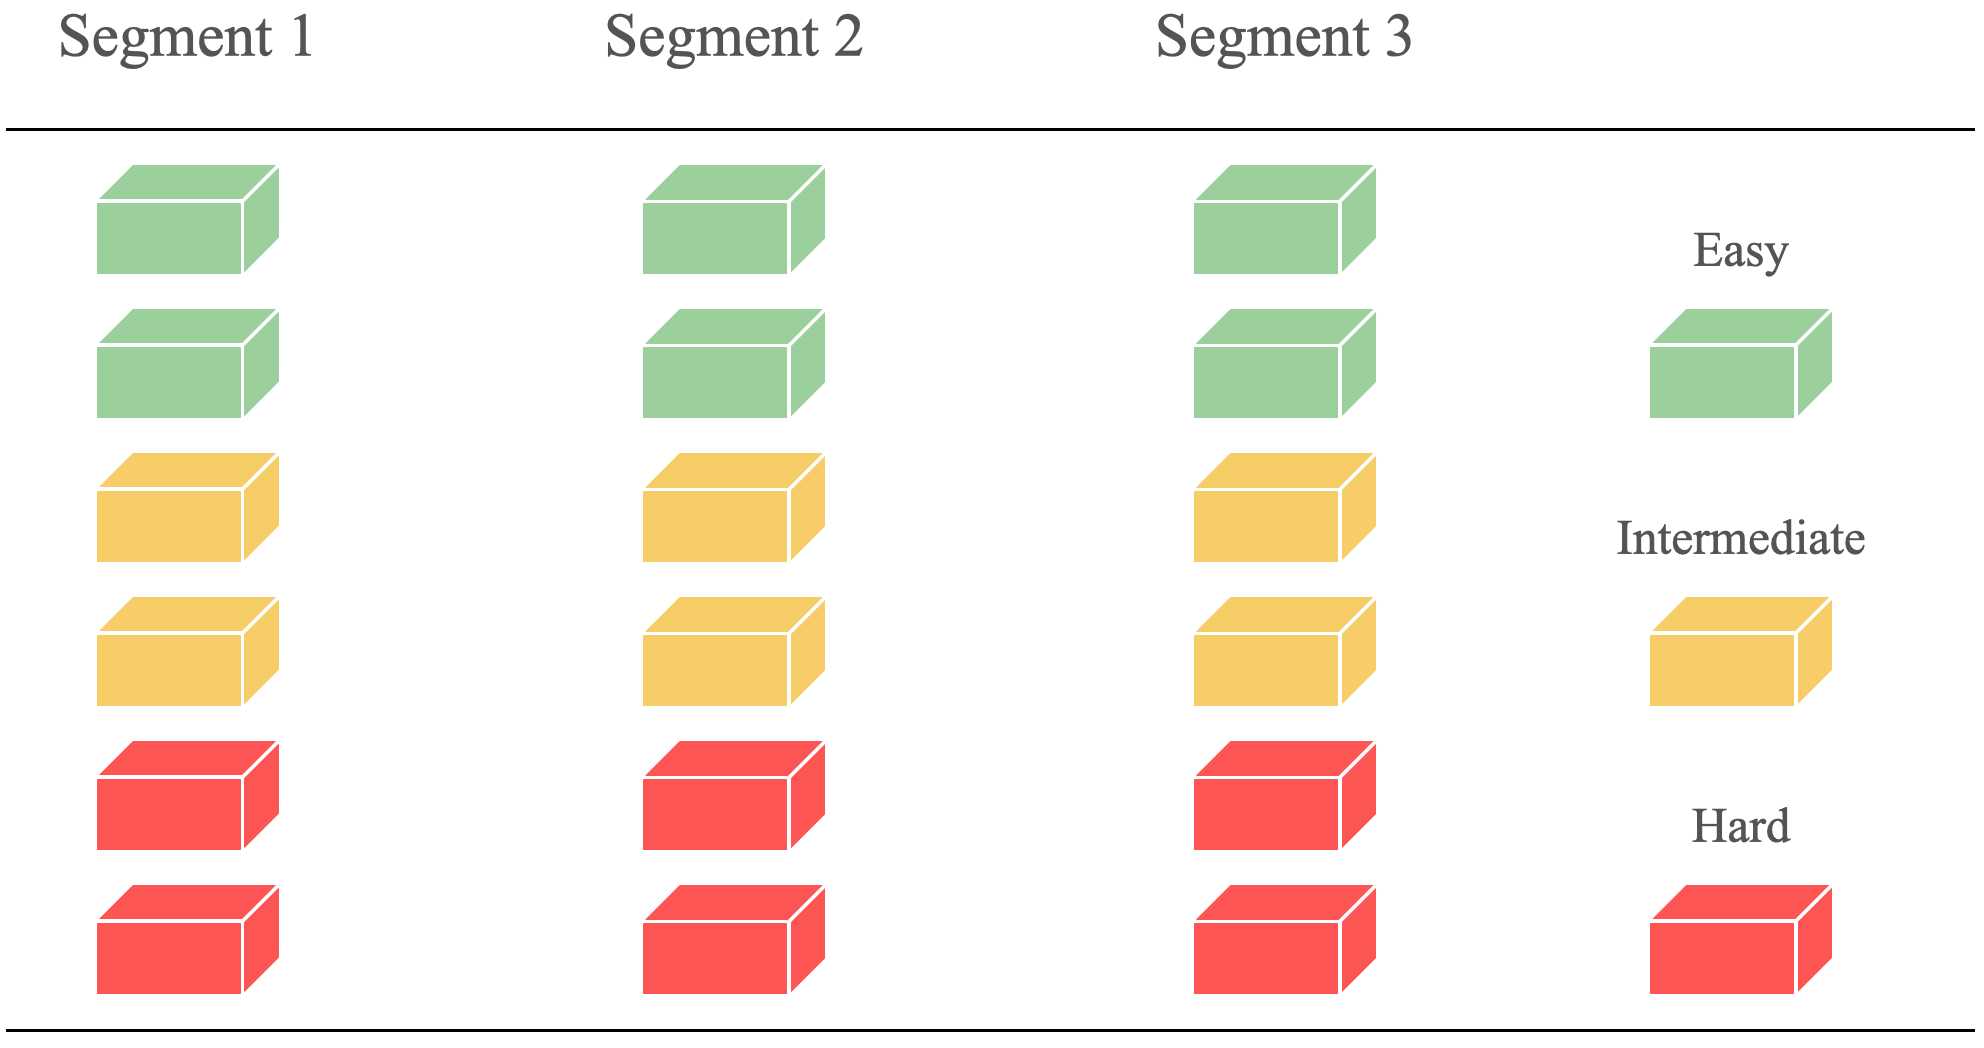
\includegraphics[scale=0.35]{experimental_setup}
\label{fig:experimental}
\bigskip
\end{figure}

The first segment emulated a scenario in which hostile spaceships approached the respondent's spaceship. The respondent was required to quickly respond by defusing the hostiles in order to survive. The increment in difficulty caused the process of defusing hostile spaceships to become more challenging, hereby aiming to cause an increase in workload. The second segment emulated a scenario in which the respondent had to navigate their spaceship trough space, gathering as many way-points as possible. Obstacles around which the respondent had to navigate carefully, as well as hostile spaceships the respondent had to decimate, were introduced in the higher difficulty sessions. The third and final segment emulated a machine room, in which respondents had to control the power based on randomly generated requests. In the increased difficulty settings, variables that could overheat the spaceship were introduced, demanding the respondent to multi-task and aiming to increase workload as a consequence.

\subsubsection{Participants}
After having to omit 7 participants due to hardware failure, 27 respondents were included in the final analysis.  18 participants are female whereas 9 are male. The mean age and standard deviation are $\mu =26, \sigma = 10.31$ respectively. The participants are students recruited from the University of Twente, as well as several employees of Thales group Hengelo. 

\subsubsection{Devices and Synchronization}
The Shimmer3 GSR+ sensor was used for both PPG and GSR measurements. This device is worn on the wrist. Signals are communicated wirelessly via Bluetooth. An ear-clip is utilized for measuring PPG. The Shimmer3 GSR+ automatically converts measured PPG signals to heart-rate. Skin conductivity, or GSR, is measured by two electrodes attached to the fingers \cite{shimmer}. EEG measurement was conducted with the Muse 2, which is a commercially offered multi-sensor headband that provides feedback on brain activity \cite{muse}. The Muse 2 headband constitutes five sensors, each monitoring a different brainwave frequency.  

The Shimmer3 GSR+ measures signals on a sampling rate of 256 Hz, whereas the Muse 2 measures at a sampling rate of 220 Hz. Given that multiple devices are utilized, data streams are required to be properly synchronized. This was accomplished by means of an application called Lab-Streaming Layer, hereafter referred to as "LSL", developed by \citeA{kothe2018lab}. The three data streams stemming from the two devices were all streamed to LSL during the experiment. LSL subsequently properly synchronizes all data streams in real-time,  such that they are parallel, hence all referring to equivalent points in time. 

\subsection{Related Work} 
The following section provides an overview of preceding research regarding the assessment of workload by means of physiological bio-signals, with a focus on deep learning approaches. Attention is predominantly placed upon the most feasible network architectures, in addition to a range of model optimization techniques and to the data fusion strategy for the multi-modular DNN. The final part of this section will be dedicated to hyperparameter optimization.  

\subsubsection{Electroencephalography (EEG)}
An overview of the complete literature on EEG applications with deep-learning was presented by \citeA{craik2019deep}, who reported a total of 16 \% of all publications to consider workload assessment specifically. The lion's share of these publications utilized either a deep belief networks or convolutional neural network, hereafter referred to as "ConvNet". One of these approaches is encouraged by the authors consequently \cite{craik2019deep}.

\citeA{tabar2016novel} proposed a hybrid of a ConvNet with a stacked auto-encoder network, hereafter referred to as "SAE network". Inputs were specified to feed into the convolutional-part with the objective of learning extracting features. The output of this part was subsequently specified to feed into the SAE part of the network,  which encompasses a stack of dense-layers, designed specifically as an input layer, six hidden layers and an output layer. A classification accuracy of 90 \% was acquired with this network \cite{tabar2016novel}. 

Research by \citeA{schirrmeister2017deep} contrasted the performance of several ConvNets against the widely utilized baseline method for EEG classification, filter bank common spatial pattern, hereafter referred to as "FBCSP". A deep ConvNet, a shallow ConvNet, a deep-shallow hybrid ConvNet and a residual ConvNet were contrasted with an FBCSP. Both the deep and shallow ConvNets were found to reach at least similar, and in some regards better classification results as compared with the FBCSP baseline approach. Altogether, a deep ConvNet with four convolutional-max-pooling blocks was found to perform best, exhibiting an accuracy of 92.4 \% \cite{schirrmeister2017deep}.

\subsubsection{Galvanic Skin Response (GSR)}
\citeA{sun2019hybrid} explored the most suitable approach to the classification of several emotional states with GSR. Various models were explored, amongst others a support vector machine, a ConvNet and a long-short-term-memory, hereafter referred to as "LSTM", network. Additionally, the feasibility of a hybrid DNN, combining both the ConvNet and LSTM approaches, was explored. This aforementioned hybrid model was found to perform best, exhibiting an accuracy of 74\% \cite{sun2019hybrid}. 

\citeA{dolmans2020perceived} took, amongst other approaches to workload prediction,  a GSR approach, and designed a variant based on the previously delineated CovNet-LSTM structure. The performance of this model was contrasted with a network consisting solely of fully connected dense layers. Conform with findings by  \citeA{sun2019hybrid}, the hybrid model was found to perform best, displaying an absolute difference between predicted and true label of 0.197 (scaled on 0-1). The model architecture as utilized deployed two convolutional max-pooling blocks and two LSTM layers \cite{dolmans2020perceived}.

\subsubsection{Photoplethysmography (PPG)}
Research by \citeA{biswas2019cornet} explored a deep learning approach towards PPG classification, with the objective to perform both bio-metric identification and obtain heart rate information. Exceptional results were realized with a DNN, attaining an average accuracy of 96 \% \cite{biswas2019cornet}. This performance was realized with a ConvNet-LSTM hybrid, incorporating two convolutional max-pooling blocks followed by two LSTM layers. 

\subsubsection{Multi-modular Fusion Strategy}  
When conducting a multi-modular deep learning approach,  information streams stemming from the different modalities are required to be combined, i.e. "fused", at a certain point in the network in order to ultimately result in a single prediction of workload. Fusion can be done conforming several strategies. Three strategies as proposed by \citeA{ramachandram2017deep} have been considered.

Early, or data-level, fusion constitutes an approach that fuses data sources before being fed into the network. Early fusing is usually proven to be quite challenging, residing in the fact that data streams stemming from different modalities often differ in their dimensionality and sampling rate. In addition, when taking an early fusion approach, the oversimplified assumption of conditional independence is made implicitly. This assumption is unrealistic in nature, for data stemming from different modalities are expected to be correlated in practice \cite{ramachandram2017deep}. 

Late, or decision-level, fusion refers to the process of aggregating the decisions of multiple separate networks, each applied towards every modality separately. In case the data sources stemming from the various modalities are either correlated or ultimately differ in their dimensionality, late fusion is often a more feasible approach as opposed to early fusion \cite{ramachandram2017deep}.

Lastly, intermediate fusion is the most widely employed fusion strategy for multi-modular deep-learning problems. Data streams are usually fused by a concatenation layer, joining the outputs of the separately defined network parts of each modality. This results in a single joint deep neural network. Several "higher-order layers" are usually defined in between the concatenation layer and the ultimate classification. The depth of the fusion, i.e. the specified number of higher-order layers, can be chosen conform to the specific circumstances, posing intermediate fusion to be the most flexible and therefore the most widely adopted fusion strategy \cite{ramachandram2017deep}.

Indeed, when consulting the literature, one is prone to conclude that intermediate fusion strategies are the most prevailing for multi-modular deep learning approaches. When taking an intermediate fusion approach, the higher-order part of the network needs to be designed and established, for which several previous research endeavors are considered.  \citeA{rastgoo2019automatic} utilized a multi-modular ConvNet approach, and fused the modalities by concatenation, followed with two LTSM layers and two dense layers. A simpler approach is adopted by \citeA{han2020classification}, who utilized an intermediate fusion approach solely consisting of several fully connected dense layers. Lastly, \citeA{dolmans2020perceived} took a relatively deep intermediate fusion approach, consisting of two dense layers, two convolutional layers followed by another two dense layers.  

\subsubsection{Model Optimization Strategies}
The technique of batch normalization was initialized by \citeA{ioffe2015batch}, and is widely utilized in DNN's with the objective of stabilization. Especially ConvNets benefit from this technique. It is beneficial to incorporate a batch normalization layer subsequent to a convolutional layer, but before feeding into the activation function \cite{ioffe2015batch}.  All previously delineated networks architectures utilize batch normalization layers, in most cases specified subsequent to each convolutional layer \cite{dolmans2020perceived} \cite{tabar2016novel} \cite{schirrmeister2017deep} \cite{biswas2019cornet} \cite{sun2019hybrid}.

Pooling layers are commonly employed in ConvNets, usually succeeding a convolutional layer with the purpose of reducing dimensionality. The objective of such layers are to down-sample features into a more compact space, hereby only retaining indispensable information. For a more extensive elaboration on pooling, please consult \citeA{lecun2015deep}. All previously delineated networks architectures utilize max-pooling layers, usually specified subsequent to the activation layer \cite{dolmans2020perceived} \cite{tabar2016novel} \cite{schirrmeister2017deep} \cite{biswas2019cornet} \cite{sun2019hybrid}.

\subsubsection{Hyper Parameter Optimization}
Hyper parameter optimization, hereafter referred to as "HPO", is a technique that can be utilized to optimize network hyper-parameters, such as learning rate and dropout rate.  In theory, one could optimize the entire DNN architecture, including the number of neurons/filters in (convolutional) layers, the number of layers in general, whether to use certain layers etc. There is, however, a strong relationship between the amount of parameters to be optimized and the computational resources required to do so, in where many parameters to optimize tends to inflate computational costs by a substantial amount. Substantial advancements in DNN performance have been attained by utilizing HPO, especially for ConvNets \cite{bergstra2012random}. The Optuna toolbox provides a method for creating a parameter search space, from which values for the hyper-parameters can be sampled and optimization can be performed \cite{akiba2019optuna}. 
\bigskip 

\subsection{Deep Neural Network Architectures \& Training} \label{section:DNN}
Before elaborating on the chosen DNN architectures, we will firstly touch upon several universal truths for all networks.  Given the person-specific character inherent to physiological data,  networks for each respondent have been trained independently. Despite this, all network architectures across persons are similar, except for the specified hyperparamaters: these were optimized for each of the four networks and for each respondents individually as well. As a consequence, four DNN's are trained for each of the 27 respondents separately, resulting in a total of 108 trained networks, each one utilizing one of 108 sets of optimized hyperparamaters. All networks were 

\subsubsection{Single-modular Network}
All single-modular network architectures took inspiration from previously delineated research \cite{schirrmeister2017deep} \cite{dolmans2020perceived} \cite{sun2019hybrid} \cite{biswas2019cornet}. In contrast with most of these previous endeavors, we opted for a ConvNet-only approach, i.e. without LSTM-layers, for the objective of the current research is not of a time-series-forecasting-kind. An experimental scenario wherein the course of actions over the duration of the experiment always unfold in a similar manner are inclined to benefit from acknowledging this time-series-like nature, hence benefiting from LSTM. An example of such a scenario would be a pilot in flight: whilst workload arousing phenomena that occur during a flight could differ across takes, the general chronological structure of the scenario always adheres to a similar blueprint. I.e., starting with ascend, likely to arouse a peak in workload, and closing with touch down, equally so likely to arouse a peak in workload. Our experimental scenario doesn't adhere to such a set in stone unfolding, for the order in which the scenario's with variable difficulty were presented was entirely randomized.  Hence, for there is no chronologically consistent development of the experimental scenario, we opted for a ConvNet approach without opting to learn from the development over time, thus without LSTM-layers.  

The three single-modular DNN architectures are depicted alongside one another as Figure \ref{fig:singlearchitecture}. Each of the single-modular networks can be distinguished by two separate part, being the convolutional part and the prediction part.  The objective of the convolutional part is to extract features from the data. For each network, this part consists of four convolutional blocks, each compromising a convolutional layer, a batch normalization layer, the Exponential Linear Unit, hereafter referred to as "ELU", activation function, and a max-pooling layer respectively. The prediction part compromises a flatten-layer,  with the objective of representing all input into one dimensional shape, followed by a dropout layer, a dense layer, a Rectified linear activation, hereafter referred to as "RELU", closed by another dense layer. An overview of the amount of utilized filters / neurons for each layer of each network is provided in Table \ref{table:modelvariations}. 

Consistent with training, HPO was equally so done for each respondent individually, resulting in 27 optimized sets of parameters for the EEG networks, 27 for the PPG networks and 27 for the GSR networks.We optimized the learning rate, dropout rate and the amount of neurons for the first dense layer in 50 trials per network.  For training, a total of 600 epochs have been made through the data for each network independently. All training and HPO of the single-modular networks has been done on a V100 GPU,  offered by the GPU cloud service Google Collab.  Total running time for the single-modular networks was about four days, the most of which was absorbed by HPO. 

\newgeometry{margin=2cm}
\begin{figure}
\caption{The Three Single-modular Network Architectures}
\bigskip
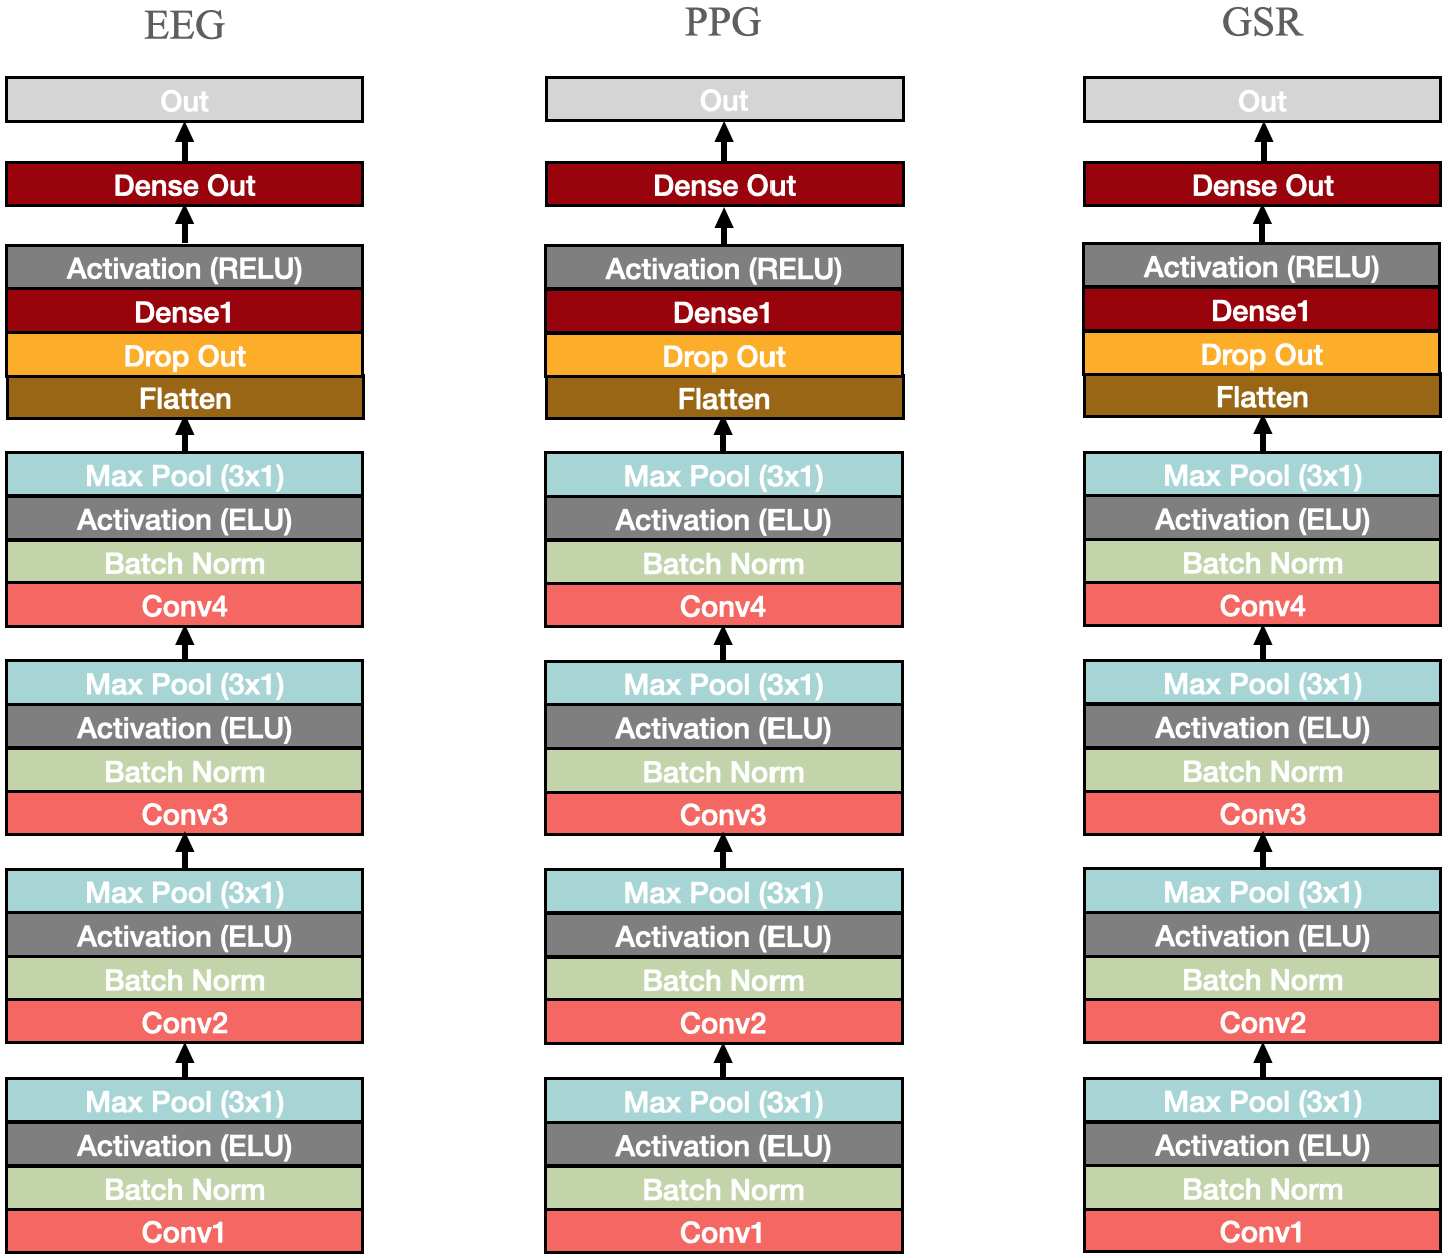
\includegraphics[scale=0.69]{single_model_architecture}
\label{fig:singlearchitecture}
\floatfoot{\emph{Note:} Each network constitutes a convolutional part of four convolutional blocks, and a classification part of two fully connected dense layers. }
\end{figure}
\restoregeometry

\newgeometry{margin=1.6cm}
\bgroup
\def\arraystretch{1.6}%  
\begin{table}[h]
\caption{Network Sizes}
\label{table:modelvariations}
\begin{tabular}{lllll}
\hline
        & EEG-Net/Part  & GSR-Net/Part  & PPG-Net/Part  & Multi-Modular Head-Net     \\ \hline
 Single-Modular-Nets & Dense Out: 1 & Dense Out: 1 & Dense Out: 1 &   \\
        & Dense 1: \emph{hpo} & Dense 1: \emph{hpo} & Dense 1: \emph{hpo} &   \\
        \vspace{1.5ex}        
        & Drop out: \emph{hpo} & Drop out: \emph{hpo} & Drop out: \emph{hpo} &   \\
        & Conv4: 200 & Conv4: 128 & Conv4: 128 &    \\ 
        & Conv3: 100 & Conv3: 64 & Conv3: 64 &    \\ 
        & Conv2 50 & Conv2: 32 & Conv2: 32 &    \\ 
        \vspace{3ex}
        & Conv1: 25 & Conv1: 16 & Conv1: 16 &  \\         
  Multi-Modular-Net & Dense 1: \emph{input} & Dense 1: \emph{input} & Dense 1: \emph{input} & Dense Out: 1  \\
        & Conv4: 200 & Conv4: 128 & Conv4: 128  &  Dense 3: \emph{hpo} \\ 
        & Conv3: 100 & Conv3: 64 & Conv3: 64 & Dense 2: \emph{hpo}  \\ 
        & Conv2 50 & Conv2: 32 & Conv2: 32 & Drop out: \emph{hpo}    \\ 
        \vspace{3ex}
        & Conv1: 25 & Conv1: 16 & Conv1: 16 &    \\   \hline
\end{tabular}
\vspace{2ex}
\begin{doublespacing}

\floatfoot{\textit{Notes:} For all convolutional layers the depicted number reflects the amount of utilized filters, whereas for dense layers it reflects the amount  of nodes.  All depicted values are the amount of filters/nodes that a respective layer outputs. \textit{input} refers to fully connected dense layers, wherein the number of outputting nodes equals the number of inputting nodes. \textit{Hpo} implies that the value for the respective layer was optimized (see first paragraph of section \ref{section:DNN})}

\end{doublespacing}
\end{table}
\egroup
\restoregeometry


\subsubsection{Multi-modular Network}
The network architecture utilized for the multi-modular approach was determined by combining the previously characterized single-modular networks with insights drawn from previous research, in particular \cite{han2020classification}. A visual representation of the multi-modular network is depicted as Figure \ref{fig:multiarchitecture}. An overview of the amount of utilized filters and neurons for each layer of the multi-modular network is provided in Table \ref{table:modelvariations}.

The network architecture for the single-modular parts of the network are separately defined entities of the multi-modular network, but are highly similar as compared with the previously delineated single-modular networks. An intermediate fusion strategy is adopted due to its highly flexible nature as compared with alternative fusion strategies. The output of all three distinct parts in the network were flattened, followed by a dense layer and RELU activation.  Flattening was nescessary such that all inputs were represented in one-dimensional space, after which concatenation was possible. The prediction part, also referred to as "Head-Network", consists of three dense layers, alternated with dropout, batch normalization and RELU activation.  

Again, consistent with training, HPO was equally so done for each respondent individually, resulting in 27 optimized sets of parameters each of the 27 multi-modular networks. We optimized the learning rate, dropout rate and the amount of neurons for the first and second dense layers in 18 trials per network.  For training, a total of 250 epochs have been made through the data for each network independently. All training and HPO has been done on a Cloud TPU v2,  offered by the GPU cloud service Google Collab Pro.  Total running time for the multi-modular networks was about 12 days, the most of which absorbed by HPO. 

\newgeometry{margin=2cm}
\begin{figure}
\caption{The Multi-modular Network Architecture}
\bigskip
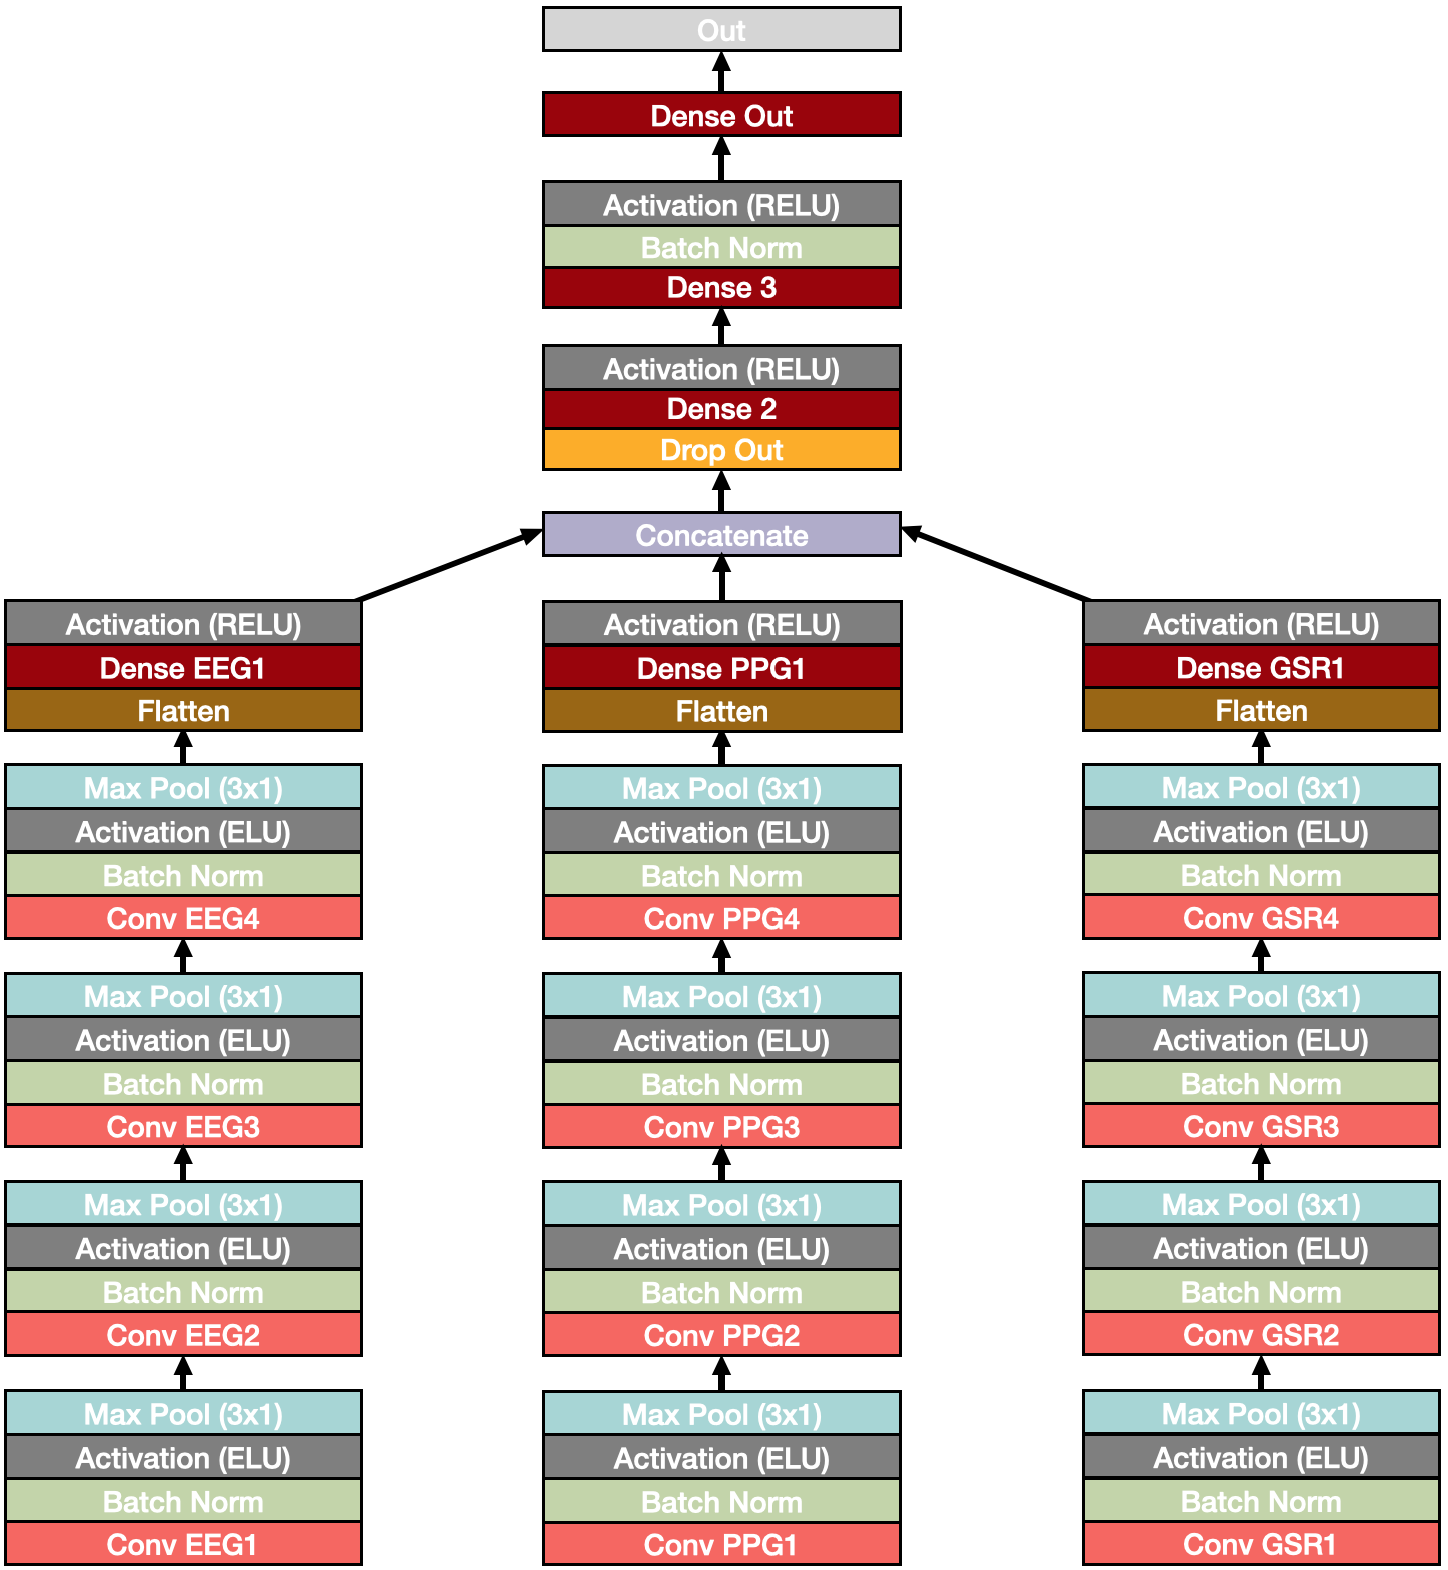
\includegraphics[scale=0.69]{multi_model_architecture}
\label{fig:multiarchitecture}
\floatfoot{\emph{Note:} The network constitutes a convolutional part of four convolutional blocks for each of distinct parts of the networks. All three distinct parts were flatenned, after which concatenation was possible.  The prediction part of the network constitutes several dense layers.}
\end{figure}
\restoregeometry

\newpage
\subsection{Model Evaluation}
The performance of the networks has been assessed and contrasted by means of several performance metrics. When assessing performance in deep/machine-learning, it is of importance to realize that each performance metric may favor one approach over the other, simply and solely due to the mathematical nature in which both the metric and the model are defined \cite{gunawardana2009survey}. For this reason, we consider a conglomerate of different metrics. 

The Mean Absolute Error, hereafter referred to as "MAE",  of a DNN is the first utilized performance metric, defined as Equation \ref{eq:mae},

\begin{equation}
\label{eq:mae}
\frac{1}{n} \sum^n_{i=1}|f(x_i)-y_i| 
\end{equation}
where $n$ refers to the amount of windows utilized for testing, $x_i$ to the predicted value for window $i$ and $y_i$ to the true label of window $i$.
The MAE constitutes the most straightforward metric for the assessment in performance of a DNN, especially since the value can simply be interpreted as the average amount by which the prediction was off.

The Root Mean Squared Error, hereafter referred to as RMSE, is the second utilized performance metric, defined as Equation \ref{eq:rmse},

\begin{equation}
\label{eq:rmse}
\sqrt{{\frac{1}{n} \sum^n_{i=1}|f(x_i)-y_i|}^2}
\end{equation}
where $n$ refers to the amount of windows utilized for testing, $x_i$ to the predicted value for window $i$ and $y_i$ to the true label of window $i$.The RMSE, which is strongly related to the MAE, differs in that it punishes big absolute differences more severely. 

Finally, the Pearson Correlation Coefficient, hereafter referred to as simply "correlation", constitutes the third utilized performance metric defined as Equation  \ref{eq:corr},

\begin{equation}
\label{eq:corr}
r_{X,Y} = \frac{cov(X,Y)}{\sigma_{X} \sigma_{Y}}
\end{equation}
where $x$ refers to the predicted values for the test windows,  $y$ to the true labels of test windows and $\sigma_{X}\, \& \,\sigma_{Y}$ refer to the standard deviation of $x$ and $y$ respectively.  Conceptually, correlation indicates the coherence between predictions and labels, hereby posing an alternative model performance metric. 

\newpage
\section{Results}
Before illustrating results,  a short elaboration on the testing procedure will be provided.  Windows of eight seconds each were cut, resulting in a total of 9474 windows over all respondents, i.e. on average about 351 windows per respondent. For each network for each respondent individually,  80\% of all windows have been used for training, 10\% for validation within the training process and 10\% for the assessment of performance. This results in an average of 35 windows for assessing DNN performance per respondent, i.e. a total of 969 windows in total.  Partitioning windows into train-, validation- and testing -sets was done systematically by selecting every \textit{n-th} window, such that windows over the entire duration of the experiment were represented equally in each partition.  These partitions compromise exactly the same windows across the four networks. 

The distribution of all 9474 window labels, aggregated for all respondents,  is depicted as Figure \ref{fig:labels}. It becomes readily apparent that distribution of the window labels displays a noticeably right-skewed tendency, with a median of 5.75 and a 12.75 90\% upper-bound quantatile, implying that higher workload windows are relatively uncommon within both train and test partitions.  
\vspace{0.1cm}

\begin{figure}[h]
\caption{Distribution Window Labels}
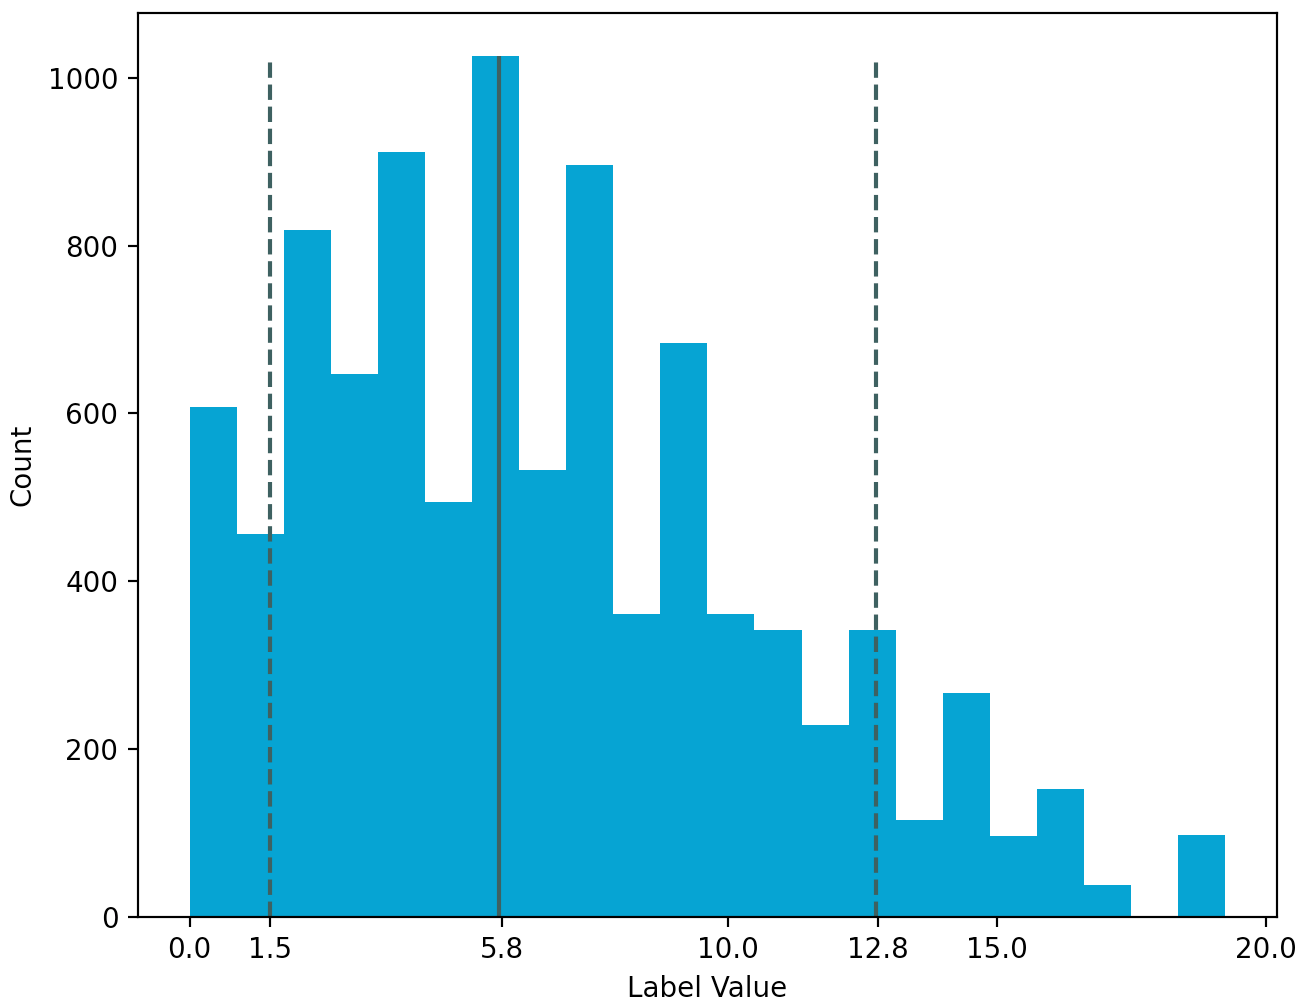
\includegraphics[scale=0.39]{labels.png}
\label{fig:labels}
\floatfoot{\emph{Note:} The solid line represents the median, whereas the two dashed line represent the 10\% and 90\% quantiles respectively.}
\end{figure}

\subsection{Deep Neural Network Performance}
Depicted in Table \ref{table:results} are the performance metrics for each of the trained DNN's. The most conspicuous result that becomes apparent is that the multi-modality networks performs consistently worse on all metrics as compared with both the single-modular EEG and GSR networks.

\vspace{0.3cm}
\bgroup
\def\arraystretch{1.6}%  
\begin{table}[h]
\caption{Deep Neural Network performance metrics}
\label{table:results}
\begin{tabular}{lllll}
\hline
                                                                               & EEG\hspace{0.5cm} & PPG\hspace{0.5cm} & GSR\hspace{0.5cm} & Multi\hspace{0.5cm} \\ \hline
\begin{tabular}[c]{@{}l@{}}Mean Absolute Error\\ \hspace{1.2cm}(\textit{0-1 scale})\end{tabular} & 0.110 & 0.136 & 0.119 & 0.128  \\
\begin{tabular}[c]{@{}l@{}}Mean Absolute Error\\ \hspace{0.25cm}(\textit{original 0-20 scale})\end{tabular} & 2.206 & 2.717 & 2.377 & 2.570 \\
Root Mean Square Error                                                         & 0.154 & 0.180 & 0.159 & 0.167 \\
Pearson Correlation                                                                    & 0.688 & 0.530 & 0.653 & 0.609 \\ \hline
\end{tabular}
\end{table}

Performance in terms of MAE of the EEG networks is superior over all other networks, with $MAE = 0.110$ with a standard deviation of $\sigma = 0.154$.  The DNN's demonstrating the next best performance are the GSR networks, closely pursuing the EGG networks,  and displaying $MAE = 0.119$ with a standard deviation of $\sigma = 0.159$.  Surprisingly, the multi-modular networks check out on the third place, displaying $MAE = 0.128$ with a standard deviation of $\sigma = 0.167$.  The PPG networks can clearly be considered the worst performing networks, displaying $MAE = 0.136$ with a standard deviation of $\sigma = 0.179$.  

A similar pattern can be observed when observing the RMSE.This is not surprising, given the RMSE is very similar to the MAE. The difference is that the RMSE values for all networks reside slightly higher, which is not surprising for the punishes high deviations more severely. 

The correlation between predictions and labels are indicative of a similar pattern as compared with the other metrics. Although patterns are similar, an interesting disparity is, however, that the differences across the four architectures is more substantial. The value for the EEG networks are observed to be $r=0.688$, which is interpretable as a rather strong correlation. Equally so, the GSR networks display a fairly strong correlation of $r=0.653$. Again, Both the multi and GSR networks are the least accurately performing, displaying a correlation of $r=0.609$ and $r=530$ respectively. 

A graphical visualization of the prediction errors for each of the four network architectures is depicted as Figure \ref{fig:mae_hist}. 

\vspace{0.3cm}
\begin{figure}[h]
\caption{Error per modality}
\bigskip
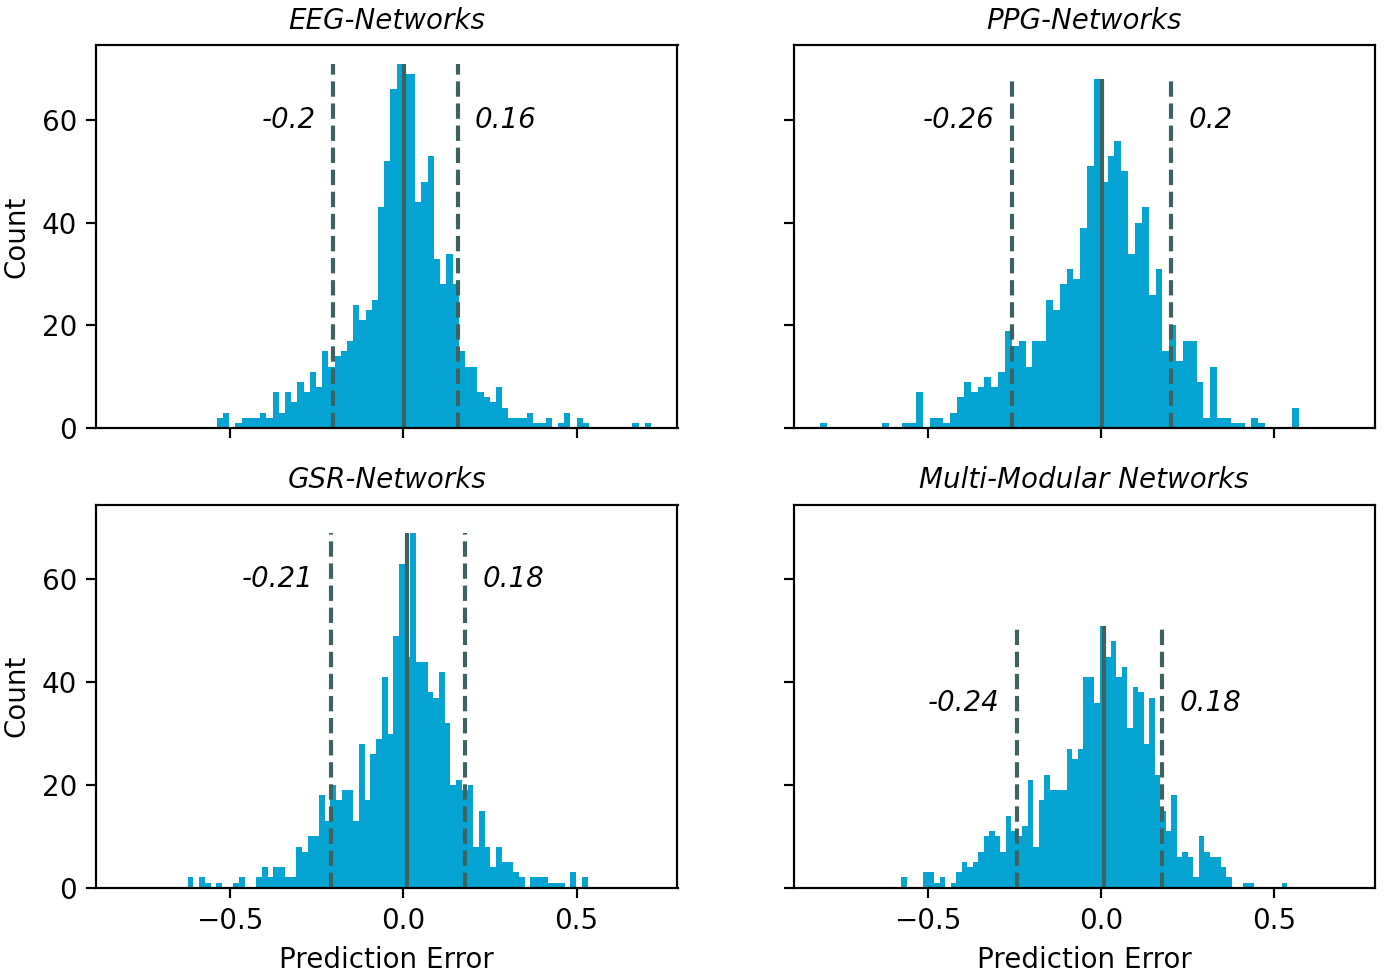
\includegraphics[scale=0.6]{error_hist.png}
\label{fig:mae_hist}
\floatfoot{\emph{Note:} The solid line represents the medians, whereas the two dashed line represent the 10\% and 90\% quantiles respectively. The displayed numbers are the values of the quantiles.}
\end{figure}

In line with the previously delineated results, it becomes readily apparent that the distribution of the prediction errors for the EEG networks approximates the normal distribution most closely, as indicative by the strong accumulation around 0 error and relatively flat tails. Not surprisingly, the two worst performing DNN's, being the multi-modular and PPG networks, display much thicker tails, and are observed to have a less accumulation around the 0 error mark (i.e. visually "less-peaked"). This is equally so demonstrated by the 10\% and 90\% quantiles, residing farthest from the median.  All distributions are observed to be slightly left-skewed, as indicated firstly by shape and secondly by the fact that 10\% quantiles are farther removed from the median as compared with the 90\% quantiles. Despite that this left-leaning tendency is observable for all network architectures, it is most profound for the PPG and multi-modular networks.  These previously delineated anomalies indicate that all networks are less accurate in predicting high-labeled windows, and that this seems to be more profound for the PPG and multi-modular networks.

Figure \ref{fig:mae_scatter} helps explore this notion into more detail,  by plotting prediction error of each window against its label value,  in addition to their linear relationship and correlation coefficient.

\vspace{0.3cm}
\begin{figure}[h]
\caption{Window Prediction Error as opposed to Window Label Value}
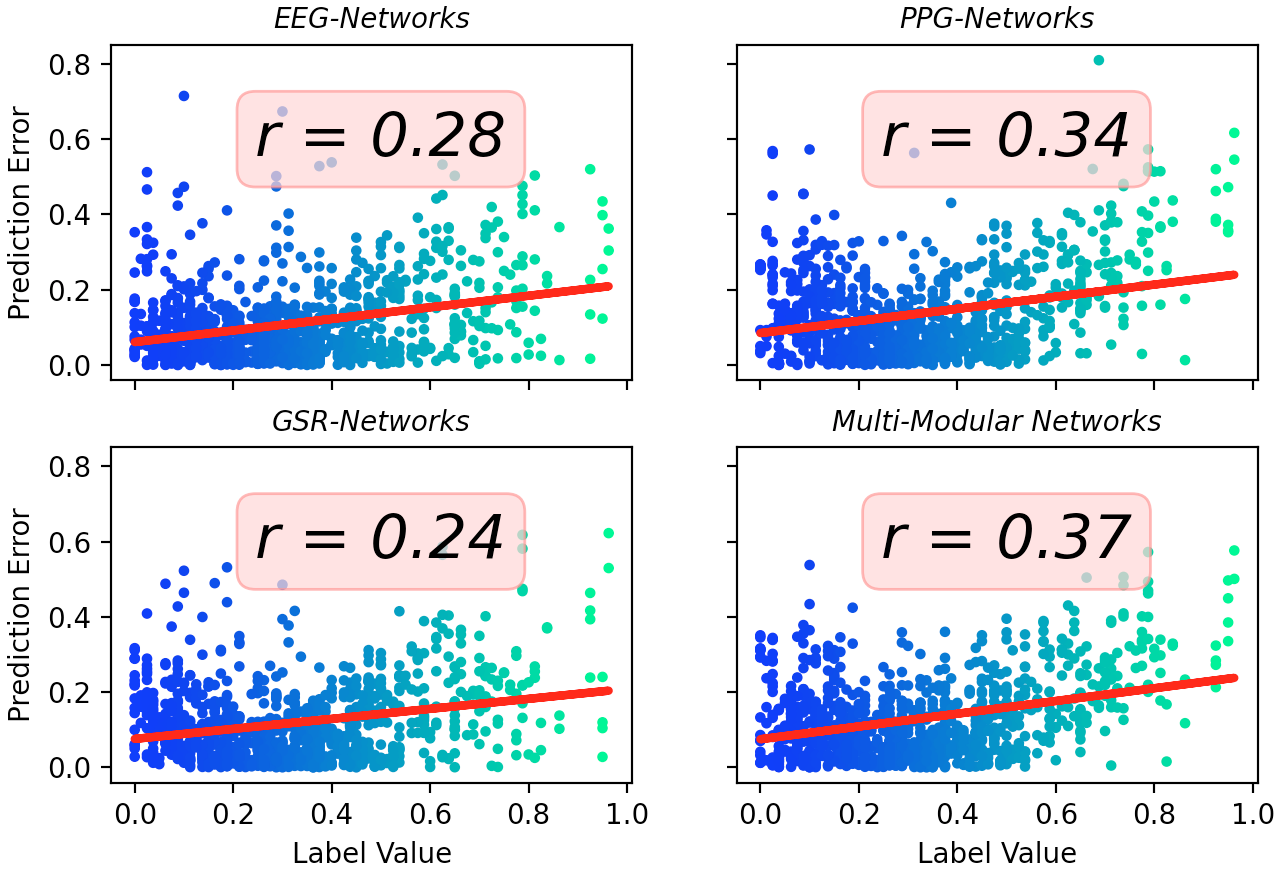
\includegraphics[scale=0.64]{mae_scatter.png}
\label{fig:mae_scatter}
\floatfoot{\emph{Note:} The red lines represent the linear relationship between prediction error and label value. The values \textit{r} represent their Pearson Correlation Coefficient.}
\end{figure}

Firstly, it becomes immediately apparent that higher labeled windows are substantially less prevailing, as indicative by the thin spreading of dots for the higher labels, conform to the conclusion drawn from the earlier depicted Figure \ref{fig:labels}. Noteworthy is that, for each the four network architectures, a relationship can be observed between the height of the absolute value of the prediction error and the height of the label. This is indicative by the moderately ascending slope, as well as the correlation coefficients. Substantively, this implies that all network architectures are observed to be considerably less accurate when predicting high labeled windows.  This tendency upholds the most for the multi-modular and PPG networks, with an observable correlation coefficients as high as $r=0.37$ for the multi-modular networks specifically.  A, less severe, but still noteworthy relationship between prediction error and label size is observable for both the GSR and EEG architectures,  with a correlation coefficients of $r=0.24$ and $r=0.28$ respectively.

\section{Conclusion and Discussion}
It can be concluded that the single-modular EEG networks consistently exhibit the best performance,  with a rather noteworthy difference on the correlations in particular.  The single-modular GSR networks, although being worse as compared with the EEG networks, also were observed to exhibit fairly adequate performance.  Most surprising is that the multi-modular networks performed substantially worse as the previously mentioned, especially as compared with the EEG networks. This was not expected, for one is enticed to expect that the network combining information from multiple modalities would yield more adequate performance as compared with networks solely using a single of these modalities. Apparently  

\begin{itemize}
  \item  More HPO could have been done, to get even better performing models but we had limited computatioal power.   
  \item This approach costs a lot of computational power to both train and do HPO. Especially since person-specific models are fitted. This upholds mostly for the multi-modal network.
  \item Due to the sheer size of the trained model and the fact that models are trained person specific, storage sizes of the models are huge. This could be unpractical.  This upholds mostly for the multi-modal network.
  \item Possibly different window sizes per modality could lead to better results.  * Insert some of the sources here that suggest different window sizes per modality* . This was beyond the scope of this project.
   \item How generizable is this to other situations for the same person (since things such as PPG are context dependent (like for example regarding how one ate).
   \item Long runtimes,  even when testing. This upholds only for the multi network. The reason is likely the sheer size of these networks, which for some persons are blown up due to device lagging. 
   \item hardware failure?
   \item The fact that we use TLX as labels.
\end{itemize}





\newpage
\bibliographystyle{apacite}
\bibliography{References}

\end{document}
